\section{Theorie}
\label{sec:Theorie}
Die Inhalte des Theorieteils sind auf Grundlage von Dokument \cite{V353} formuliert.
In der elektrischen Schaltungstechnik werden RC-Kreise häufig als Tiefpässe genutzt. 
Zur Beschreibung des Verhaltens eines RC-Kreises wird die Zeitkonstante $RC$ genutzt.
\subsection{Allgemeine Relaxationsgleichung}
Wird ein System aus seinem Ausgangszustand entfernt und es nicht in diesen zurück oszilliert, nennt man dies eine Relaxationserscheinung.
In diesem Versuch wird die Entladung eines Kondensators über einen Widerstand als Beispiel für ein Relaxationsphänomen gewählt.
Zunächst wird allgemein die Änderungsgeschwindigkeit einer Größe $A$ betrachtet. Diese ist meist proportional zur Abweichung der Größe $A$ vom Endzustand $A(\infty)$
\begin{equation*}
    \frac{\text{d}A}{\text{d}t}=c[A(t)-A(\infty)] \; \text{.}
\end{equation*}
Durch Integrieren und Umformen der Gleichung erhält man für $A(t)$
\begin{equation}
    A(t)=A(\infty)+[A(0)-A(\infty)]e^{ct} \, ,
\end{equation}
mit einem $c<0$, da $A(t)$ beschränkt sein muss.
\begin{figure}
    \centering
    \caption{Schaltbild der Entladung (Stellung 1) und Aufladung (Stellung 2) eines Kondensators über einen Widerstand} 
    \label{fig:auf-ent}
    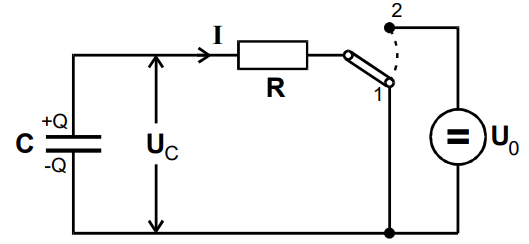
\includegraphics[width = 0.5\textwidth]{pics/auf-ent.png}
\end{figure}
\subsection{Entladevorgang eines Kondensators}
In Abbildung \ref{fig:auf-ent} sieht man den Aufbau für den Auf- und Entladezustand eines Kondensators.
Für den Versuch wurde nur der Entladevorgang genutzt, weshalb dieser auch nur in dem Theorieteil auftaucht.
Besitzt ein Kondensator mit der Kapazität $C$ eine Ladung $Q$, so liegt dort die Spannung 
\begin{equation*}
    U_\text{C}=\frac{Q}{C}
\end{equation*}
an. Mit dem Zusammenhang
\begin{equation*}
    I=\frac{U_\text{C}}{R}=- \frac{\text{d}Q}{\text{d}t}
\end{equation*}
ergibt sich für die Ladung $Q$ beim Entladevorgang, die zeitliche Differentialgleichung
\begin{equation}
    \label{eqn:Q-DGL}
    \frac{\text{d}Q}{\text{d}t}=-\frac{1}{RC}\,Q(t)\; \text{.}
\end{equation}
Bei der Entladung wird der Kondensator nach unendlich langer Zeit entladen sein. Es gilt
\begin{equation*}
    Q(\infty)=0\; \text{.}
\end{equation*}
Mit Hilfe von Integration folgt für $Q$
\begin{equation}
    Q(t)=Q(0)\exp(-t/RC)\; \text{.} \label{eqn:Charge}
\end{equation}
\subsection{Relaxationsphänomene bei angelegter Wechselspannung}
\begin{figure}
    \centering
    \caption{RC-Kreis mit Wechselspannung} 
    \label{fig:Wechs}
    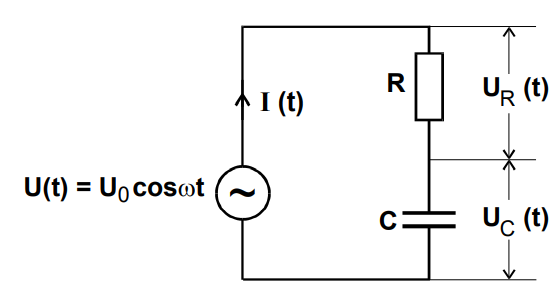
\includegraphics[width = 0.5\textwidth]{pics/wechselspannung-RC.png}
\end{figure}
Eine angelegte Wechselspannung kann wie in \ref{fig:Wechs}, als 
\begin{equation*}
    U(t)=U_0 \cos(\omega t)
\end{equation*}
dargestellt werden. Beim Vergleich der Spannungen $U(t)$ und $U_c(t)$ in Abhängigkeit von der Frequenz, bildet sich eine Phasenverschiebung $\varphi$ aus.
Somit lässt sich die ausgehende Wechselspannung als
\begin{equation}
    U_\text{C}(t)= A(\omega) \cos (\omega t + \varphi (\omega))
\end{equation}
darstellen. Dabei ist $A(\omega)$ die Kondensatorspannungsamplitude.
Mit \eqref{eqn:Q-DGL} und \eqref{eqn:strom} lässt sich $I(t)$ darstellen als
\begin{equation}
    \label{eqn:strom}
    I(t)= \frac{\text{d}Q}{\text{d}t}=C\, \frac{\text{d}U_\text{C}}{\text{d}t}\; \text{.}
\end{equation}
Durch weitere Umformungen kann die Kondensatorspannungsamplitude in Abhängigkeit dargestellt werden als 
\begin{equation}
    \label{eqn:aphi}
    A(\omega)=-\frac{\sin (\varphi)}{\omega RC}\, U_0 \, .
\end{equation}
In Gleichung \eqref{eqn:aphi} lässt sich $\varphi$ ersetzen somit ergibt sich für $A(\omega)$
\begin{equation}
    \label{eqn:ampli}
    A(\omega)=\frac{U_0}{\sqrt{1+\omega^2 R^2 C^2}} \; \text{.}
\end{equation}
Es sind mehrere Eigenschaften für $A(\omega)$ ersichtlich. Bei $\omega \rightarrow 0$ geht die Amplitude gegen $U_0$, während sie bei 
$\omega \rightarrow \infty$ verschwindet. Dies sind Eigenschaften eines Tiefpasses. Es ist auch zu erkennen, dass $A(\omega)$ nach \eqref{eqn:ampli}
nur mit $1/\omega$ gegen $0$ geht.
\subsection{Der RC-Kreis als Integrator}
Ein RC-Kreis, welcher wie in Abbildung \ref{fig:Wechs} angeschlossen ist, ist in der Lage eine zeitlich veränderliche Spannung $U(t)$ zu integrieren.
Es lässt sich zeigen, dass die Spannung $U_\text{C}$, bei Frequenzen $\omega >> \frac{1}{RC}$, proportional zu $\int U(t) \symup{dt}$ ist.
Dazu nimmt man die Maschenregel
\begin{equation}
    U(t)=U_\text{R}(t)+U_\text{C}(t) =I(t)R +U_\text{C}(t)
\end{equation}
und ersetzt $I(t)$ durch \eqref{eqn:strom} und bekommt
\begin{equation*}
    U(t)=RC\, \frac{\text{d}U_\text{C}}{\text{d}t} + U_\text{C}(t) \; \text{.}
\end{equation*}
Unter der Bedingung $\omega >> \frac{1}{RC}$ ist $|U_\text{C}| << |U_\text{R}|$ und $|U_\text{C}| << |U|$. 
Damit lässt sich näherungsweise 
\begin{equation*}
    U(t)=RC \, \frac{\text{d}U_\text{C}}{\text{d}t}
\end{equation*}
schreiben, welches durch Umformen und Integrieren zu
\begin{equation}
    U_\text{C}(t)=\frac{1}{RC} \int_0^t U(t') dt'
\end{equation}
wird.